%==============================================================================
% presentation.tex
%==============================================================================


%==============================================================================
% Configuration
%==============================================================================

% Internationalisation
\usepackage[utf8]{inputenc}
\usepackage[T1]{fontenc}
% \usepackage[ngerman]{babel}

% Different packages
\usepackage{url}
\usepackage{color,listings}
\usepackage{enumerate}
\usepackage{tabularx}
\usepackage{alltt}

% Use default Acrobat reader fonts
\usepackage{mathpazo}

% Use CM fonts (increases document size)
\usepackage{ae}

% Use images
\usepackage{graphicx}

% Configure beamer
\usetheme[secheader]{Ikhono}
\usefonttheme[onlylarge]{structurebold}
\setbeamertemplate{navigation symbols}{}

% Variables
\providecommand{\Title}{Parallel Programming}
\providecommand{\Subtitle}{Recitation Session 3}
\providecommand{\Author}{Thomas Weibel <weibelt@ethz.ch>}
\providecommand{\Institute}{Laboratory for Software Technology, \\
  Swiss Federal Institute of Technology Z\"urich}
\providecommand{\Date}{March 18, 2010}

% PDF settings
\hypersetup{
  pdftitle={\Title, \Subtitle},
  pdfauthor={\Author},
  pdfsubject={\Institute},
  pdfkeywords={parallel programming} 
}

% Titlepage
\title{\Title}
\subtitle{\Subtitle}
\author{\Author}
\institute{\Institute}
\date{\Date}

% Listings
\lstdefinestyle{Default}{
  language=Java,
  tabsize=2,
  mathescape=true,
  inputencoding=utf8,
  showstringspaces=false,
  fontadjust=true,
  basicstyle=\ttfamily,
  keywordstyle=\color{blue}\bfseries,
}
\lstset{style=Default}


%==============================================================================
% Document
%==============================================================================

\begin{document}


% Titlepage
\begin{frame}[plain]
  \titlepage
\end{frame}


\section*{Introduction}

\begin{frame}{Executive Summary}
  \begin{itemize}
  \item Java Questions?
    \begin{itemize}
    \item Please send me an email if you want me to discuss something
      specific in the recitation session
    \end{itemize}
  \item Synchronization
  \item Loop Examples
    \begin{itemize}
    \item Pre Increment
    \item Post Increment
    \end{itemize}
  \item MergeSort: How to parallelize?
  \item Performance Measurement
    \begin{itemize}
    \item Harsh realities of parallelization
    \item Amdahl's law
    \end{itemize}
  \end{itemize}
\end{frame}


\section{Last Assignment}

\begin{frame}{Outline}
  \tableofcontents[current]
\end{frame}

\begin{frame}{Solution: Questions Part 2}
  \begin{block}{Question}
    Why is it not sufficient to add the \lstinline!synchronized!
    keyword to the \lstinline!read()! and \lstinline!write()! methods
    to guarantee the specified behavior of the producer/consumer
    problem?
  \end{block}

  \vspace{\stretch{1}}

  \pause

  \begin{exampleblock}{Answer}
    Synchronization ensures that the producer and the consumer can not
    access the buffer at the same time.

    But it does not prevent the consumer to read a value more than one
    time or the producer to overwrite a value that was not read.
  \end{exampleblock}
\end{frame}

\begin{frame}{Solution: Questions Part 2}
  \begin{block}{Question}
    Would it be safe to use a boolean variable as a ``guard'' within
    the \lstinline!read()! and \lstinline!write()! methods instead of
    using the \lstinline!synchronized!  keyword?
  \end{block}

  \vspace{\stretch{1}}

  \pause

  \begin{exampleblock}{Answer}
    No, reading and writing a value is not atomic!

    Why is \lstinline!i++! is not atomic?
  \end{exampleblock}
\end{frame}

\begin{frame}{Solution: Questions Part 3}
  \begin{block}{Question}
    Would it suffice to use a simple \lstinline!synchronized(this)!
    within the \lstinline!run()! method of each the producer and the
    consumer to guard the updating of the buffer?
  \end{block}

  \vspace{\stretch{1}}

  \pause

  \begin{exampleblock}{Answer}
    No, since producer and consumer are different objects with
    different locks $\rightarrow$ no mutual exclusion guaranteed
  \end{exampleblock}
\end{frame}

\begin{frame}{Solution: Questions Part 3}
  \begin{block}{Question}
    What is the object that should be used as the shared monitor and
    therefore the object upon which the threads are
    \lstinline!synchronized()!?
  \end{block}

  \vspace{\stretch{1}}

  \pause

  \begin{exampleblock}{Answer}
    The shared instance of \lstinline!UnsafeBuffer!.
  \end{exampleblock}
\end{frame}

\begin{frame}{Solution: Questions Part 3}
  \begin{block}{Question}
    What could you have used instead?
  \end{block}

  \vspace{\stretch{1}}

  \pause

  \begin{exampleblock}{Answer}
    A dedicated shared lock object.
  \end{exampleblock}
\end{frame}

\begin{frame}{Solution: Questions Part 3}
  \begin{block}{Question}
    What are the potential advantages/disadvantages of synchronizing
    the producer/consumer over synchronizing the buffer?
  \end{block}

  \vspace{\stretch{1}}

  \pause

  \begin{exampleblock}{Advantages}
    \begin{itemize}
    \item Can use arbitrary (also unsafe!) buffers
    \item Can do things in the Producer/Consumer that need to be done
      before the other thread can use the buffer, for example print
      something to the console.
    \end{itemize}
  \end{exampleblock}

  \vspace{\stretch{1}}

  \pause

  \begin{alertblock}{Disadvantages}
    \begin{itemize}
    \item More work to do :-)
    \item More error-prone
    \end{itemize}
  \end{alertblock}
\end{frame}


\section{Loop Examples}

\begin{frame}{Outline}
  \tableofcontents[current]
\end{frame}

\begin{frame}[fragile]{Loop 1}
  \begin{lstlisting}
int j, m;

System.out.println("Loop 1");
j = 0;
while (j < 10) {
  j = j + 1;
  System.out.print(" " + j);
}
  \end{lstlisting}
\end{frame}

\begin{frame}[fragile]{Loop 2}
  \begin{lstlisting}
System.out.println("Loop 2");
j = 0;
while (j++ < 10) {
  System.out.print(" " + j);
}
  \end{lstlisting}
\end{frame}

\begin{frame}[fragile]{Loop 3}
  \begin{lstlisting}
System.out.println("Loop 3");
j = 0;
while (++j < 10) {
  System.out.print(" " + j);
}
  \end{lstlisting}
\end{frame}

\begin{frame}[fragile]{Loop 4}
  \begin{lstlisting}
System.out.println("Loop 4");
j = 0;
m = 0;
while (j++ < 10) {
  if (++m == j) {
    System.out.print("j=" + j + 
                     " m=" + m + "\n");
  }
}
  \end{lstlisting}
\end{frame}

\begin{frame}[fragile]{Loop 5}
  \begin{lstlisting}
System.out.println("Loop 5";)
j = 0;
m = 0;
while (j++ < 10) {
  if (m++ == j) {
    System.out.print("j=" + j + 
                     " m=" + m + "\n");
  }
}
  \end{lstlisting}
\end{frame}

\begin{frame}[fragile]{Loop 6}
  \begin{lstlisting}
System.out.println("Loop 6");
j = 0;
m = 0;
while (j < 10) {
  if (j == (++m)) {
    System.out.print("j=" + j + 
                     " m=" + m + "\n");
  }
  j++;
}
  \end{lstlisting}
\end{frame}

\begin{frame}[fragile]{Loop 7}
  \begin{lstlisting}
System.out.println("Loop 7");
j = 0;
m = 0;
while (j < 10) {
  if (m++ == j) {
    System.out.print("j=" + j + 
                     " m=" + m + "\n");
  }
  j++;
}
  \end{lstlisting}
\end{frame}


\section{MergeSort}

\begin{frame}{Outline}
  \tableofcontents[current]
\end{frame}

\begin{frame}{MergeSort}
  \begin{itemize}
  \item Problem: Sort a given list $l$ of $n$ numbers
  \item Example:
    \begin{itemize}
    \item Input: $9$ $8$ $7$ $6$ $5$ $4$ $3$ $2$ $1$ $0$
    \item Output: $0$ $1$ $2$ $3$ $4$ $5$ $6$ $7$ $8$ $9$
    \end{itemize}
  \end{itemize}

  \vspace{\stretch{1}}

  \pause

  \begin{exampleblock}{Algorithm}
    \begin{itemize}
    \item Divide l into two sub-lists of size $n/2$
    \item Sort each sub-list recursively by re-applying MergeSort
      \begin{itemize}
      \item End of recursion: Size of the sub-list becomes 1
      \item If size of a sub-list $> 1$ $\Rightarrow$ other sorting
        needed
      \end{itemize}
    \item Merge the two sub-lists back into one sorted list
    \end{itemize}
  \end{exampleblock}
\end{frame}

\begin{frame}{Example: Divide into sub-lists}
  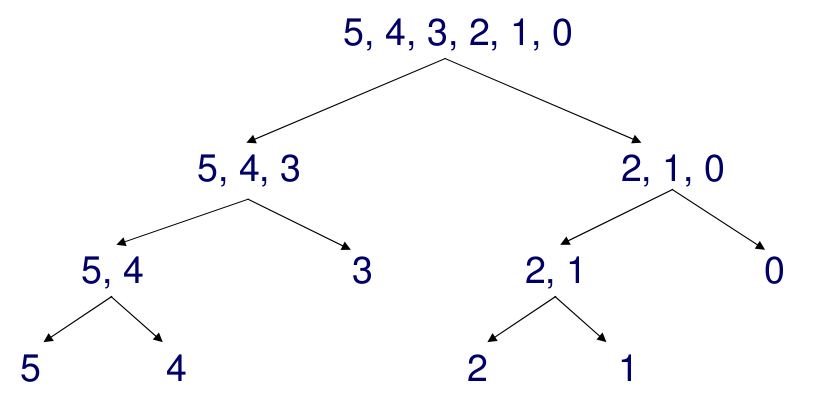
\includegraphics[width=\textwidth]{figures/mergesort-divide}  
\end{frame}

\begin{frame}{Merging}
  \begin{itemize}
  \item Combine two sorted lists into sorted list
  \item Example:
    \begin{itemize}
    \item List 1: $0$, $5$
    \item List 2: $3$, $4$, $45$
    \item Output: $0$, $3$, $4$, $5$, $45$
    \end{itemize}
  \end{itemize}

  \vspace{\stretch{1}}
  
  \begin{center}
    \begin{tabular}{c|c|l}
      List 1 & List 2 & Merged list \\\hline
      \alert{$0$}, $5$ & \alert{$3$}, $4$, $45$ & $0 < 3$ $\rightarrow$ insert $0$ in merged list: \alert{$0$} \\
      $0$, \alert{$5$} & \alert{$3$}, $4$, $45$ & $3 < 5$ $\rightarrow$ insert $3$ in merged list: $0$, \alert{$3$} \\
      $0$, \alert{$5$} & $3$, \alert{$4$}, $45$ & $4 < 5$ $\rightarrow$ insert $4$ in merged list: $0$, $3$, \alert{$4$} \\
      $0$, \alert{$5$} & $3$, $4$, \alert{$45$} & $5 < 45$ $\rightarrow$ insert $5$ in merged list: $0$, $3$, $4$, \alert{$5$} \\
      $0$, $5$ & $3$, $4$, \alert{$45$} & Finally, insert $45$ in merged list: $0$, $3$, $4$, $5$, \alert{$45$} \\
    \end{tabular}        
  \end{center}  
\end{frame}

\begin{frame}{Example: Merging sorted sub-lists}
  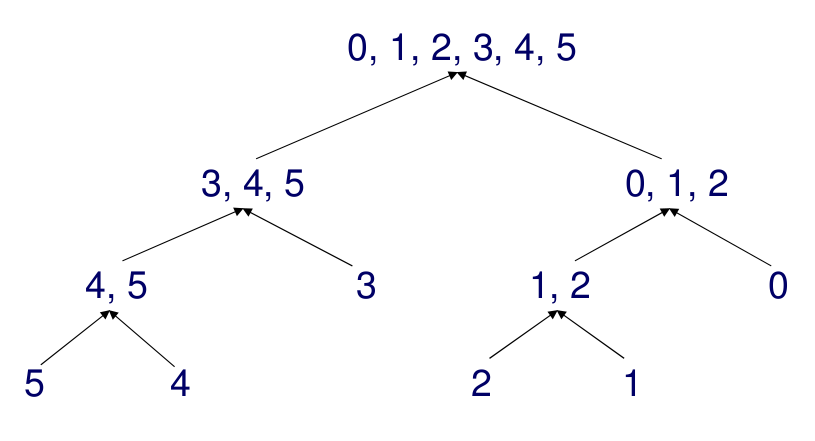
\includegraphics[width=\textwidth]{figures/mergesort-merge}  
\end{frame}

\begin{frame}{Code skeletons}
  \begin{center}
    {\huge Eclipse}
  \end{center}
\end{frame}


\section{Parallelizing MergeSort}

\begin{frame}{Outline}
  \tableofcontents[current]
\end{frame}

\begin{frame}{Which operations can be done in parallel?}
  
  \pause

  \begin{block}{Sorting}
    Each sub-list can be sorted by a separate thread
  \end{block}

  \vspace{\stretch{1}}

  \pause

  \begin{block}{Merging}
    Two ordered sub-lists can be merged by a thread
  \end{block}
\end{frame}

\begin{frame}{Parallelization issues}
  \begin{block}{Synchronization issues}
    Limitations in parallelization?

    $\hookrightarrow$ Merge can only happen if two sub-lists are sorted
  \end{block}

  \vspace{\stretch{1}}

  \begin{block}{Performance issues}
    \begin{itemize}
    \item Number of threads?
    \item Size of array to sort?
    \end{itemize}
  \end{block}
\end{frame}

\begin{frame}[fragile]{Load balancing}
  What do we do if the threads cannot be evenly distributed?
  
\begin{lstlisting}
  size of array % numThreads != 0
\end{lstlisting}

  \vspace{\stretch{1}}

  \begin{exampleblock}{Simple (proposed) solution}
    Assign remaining elements to one thread
  \end{exampleblock}

  \vspace{\stretch{1}}

  \begin{exampleblock}{Balanced (more complicated) solution}
    Distribute remaining elements to more threads
  \end{exampleblock}
\end{frame}


\section{Performance Measurement}

\begin{frame}{Outline}
  \tableofcontents[current]
\end{frame}

\begin{frame}{Performance Measurement}
  \begin{center}
    \begin{tabular}{l||c|c|c|c|c|c|c|c|c}
      & \multicolumn{9}{c}{Number of threads} \\
      Array size & 1 & 2 & 4 & 8 & 16 & 32 & 64 & \ldots & 1024 \\\hline\hline
      $100'000$ & & & & & & & & & \\\hline
      $500'000$ & & & & & & & & & \\\hline
      \ldots & & & & & & & & & \\\hline
      $10'000'000$ & & & & & & & & & \\\hline
    \end{tabular}
  \end{center}
\end{frame}

\begin{frame}[fragile]{How to measure time?}
  \begin{lstlisting}[basicstyle=\fontsize{7}{9}\selectfont\ttfamily]
public class StopWatch {
  private long startTime = 0; 
  private long stopTime = 0;
  private boolean running = false;

  public void start() {
    this.startTime = System.currentTimeMillis();
    this.running = true;
  }
  
  public void stop() {
    this.stopTime = System.currentTimeMillis();
    this.running = false;
  }
  
  public long getElapsedTime() {
    if (running) {
      return System.currentTimeMillis() - startTime;
    } else {
      return stopTime - startTime;
    }
  }
}
  \end{lstlisting}
\end{frame}

\begin{frame}{Measure time}
  \begin{itemize}
  \item \lstinline!System.currentTimeMillis()! might not be exact
    \begin{itemize}
    \item Granularity might be higher than a millisecond
    \item Might be slightly inaccurate
    \end{itemize}
  \item \lstinline!System.nanoTime()!: Nanosecond precision, but not
    nanosecond accuracy
  \item For our measurements \lstinline!System.currentMillis()! is
    good enough
  \end{itemize}
\end{frame}

\begin{frame}{$K$-Best Measurement Scheme}
  \begin{itemize}
  \item Measure the $K$ best execution times of the program
  \item $K$ measurements should be close to the best performance value
  \item Three parameters required:
    \begin{itemize}
    \item Number of measurement ($K = 3$)
    \item How close the measurements should be ($\epsilon = 5\%$)
    \item The maximum number of measurements/time before we give up
    \end{itemize}
  \item In the table: arithmetic average of measured values
  \end{itemize}
\end{frame}

\begin{frame}{Questions to be answered}
  \begin{itemize}
  \item Is the parallel version faster?
  \item How many threads give the optimum performance?
  \item What is the influence of the CPU model/CPU frequency?
  \end{itemize}
\end{frame}


\section{The Harsh Realities of Parallelization}

\begin{frame}{Outline}
  \tableofcontents[current]
\end{frame}

\begin{frame}{The Harsh Realities of Parallelization}
  \begin{exampleblock}{Ideally}
    Upgrading from uni-processor to $n$-way multiprocessor should
    provide an $n$-fold increase in computational power
  \end{exampleblock}

  \vspace{\stretch{1}}

  \begin{alertblock}{Real world}
    Most computations cannot be efficiently parallelized 

    $\hookrightarrow$ Sequential code, synchronization, communication
  \end{alertblock}

  \vspace{\stretch{1}}
\end{frame}

\begin{frame}{Speedup}
  \begin{center}
    \huge
    \begin{math}
      \text{Speedup} = \frac{\text{time}(\text{single
          processor})}{\text{time}(n \text{ concurrent processors})}
    \end{math}    
  \end{center}

  \vspace{\stretch{1}}

  \begin{block}{Amdahl's Law}
    Speedup of any complex job is limited by how much of the job must
    be executed sequentially    
  \end{block}
\end{frame}

\begin{frame}{Amdahl's Law}
  \begin{center}
    \huge
    \begin{math}
      S = \frac{1}{\underbrace{1 - p}_{\text{serial}} + \underbrace{\frac{p}{n}}_{\text{parallel}}}
    \end{math}
  \end{center}

  \vspace{\stretch{1}}

  Parameters

  \begin{itemize}
  \item $1$: normalized sequential execution time
  \item $p$: fraction that can be executed in parallel
  \item $n$: number of processors
  \end{itemize}
\end{frame}

\begin{frame}{Example}
  \begin{block}{Question}
    5 painters, and 5 rooms, 4 small rooms have the same size, one big
    room has twice the size of a small room.

    What is the speedup?
  \end{block}

  \vspace{\stretch{1}}

  \pause

  \begin{exampleblock}{Solution}
    $n = 5$, $p = \frac{5}{6}$, $1 - p = \frac{1}{6}$
    \begin{center}
      \huge
      \begin{math}
        S = \frac{1}{1 - p + \frac{p}{n}} = \frac{1}{\frac{1}{6} +
          \frac{1}{6}} = 3
      \end{math}
    \end{center}
  \end{exampleblock}
\end{frame}

\begin{frame}{Even worse?}
  \begin{block}{Question}
    10 painters, and 10 rooms, 9 small rooms have the same size, 1 big
    room has twice the size of a small room.

    What is the speedup?
  \end{block}

  \vspace{\stretch{1}}

  \pause

  \begin{exampleblock}{Solution}
    $n = 10$, $p = \frac{10}{11}$, $1 - p = \frac{1}{11}$
    \begin{center}
      \huge
      \begin{math}
        S = \frac{1}{1 - p + \frac{p}{n}} = \frac{1}{\frac{1}{11} +
          \frac{1}{11}} = 5.5
      \end{math}
    \end{center}
    $\hookrightarrow$ Even if we manage to parallelize 90\% of the
    application, but not the remaining 10\% we end up with a five-fold
    speedup
  \end{exampleblock}
\end{frame}


\section*{Outro}

\begin{frame}{Summary}
  \begin{itemize}
  \item Please send me your questions and remarks
  \item Synchronization
  \item Pre and Post Increment
  \item MergeSort and parallel MergeSort
  \item How to measure time in Java
  \item Amdahl's law
  \end{itemize}

  \vspace{\stretch{1}}

  \begin{center}
    
\includegraphics[scale=0.35]{figures/dilbert-1}
  \end{center}
\end{frame}

\end{document}
